\documentclass[12pt, a4paper]{article}

% ── Packages ──────────────────────────────────────────────────────
\usepackage{fontspec}
\setmainfont{Arial}
\usepackage{amsmath, amssymb, amsthm}
\usepackage{mathtools}
\usepackage{enumitem}
\usepackage{tikz}
\usetikzlibrary{calc, positioning, arrows.meta, fit, patterns, decorations.pathreplacing, shapes.geometric}
\usepackage{geometry}
\geometry{margin=2.4cm}
\usepackage{xcolor}
\usepackage{tcolorbox}
\tcbuselibrary{theorems, skins, breakable}
\usepackage{booktabs}
\usepackage{colortbl}
\usepackage{hyperref}
\hypersetup{colorlinks=true, linkcolor=blue!60!black, urlcolor=blue!60!black}

\setlength{\parindent}{0pt}
\setlength{\parskip}{6pt}

% ── Colours ───────────────────────────────────────────────────────
\definecolor{setA}{RGB}{66, 133, 244}   % blue
\definecolor{setB}{RGB}{234, 67, 53}    % red
\definecolor{setC}{RGB}{251, 188, 4}    % yellow
\definecolor{newEdge}{RGB}{39, 174, 96} % green for added edges
\definecolor{diagGray}{gray}{0.85}      % matrix diagonal shading
\definecolor{mirrorBlue}{RGB}{173,216,230}  % mirrored pair highlight (light blue)
\definecolor{mirrorRose}{RGB}{255,204,204}  % mirrored pair highlight (light rose)
\definecolor{theoryBg}{RGB}{232, 245, 253}
\definecolor{theoryFrame}{RGB}{66, 133, 244}
\definecolor{stmtBg}{RGB}{255, 243, 224}
\definecolor{stmtFrame}{RGB}{230, 126, 34}
\definecolor{ansBg}{RGB}{232, 250, 232}
\definecolor{ansFrame}{RGB}{39, 174, 96}

% ── Environments ──────────────────────────────────────────────────
\newtcolorbox{theorybox}[1][]{%
  colback=theoryBg, colframe=theoryFrame,
  fonttitle=\bfseries, title={\small Տեսության ամփոփում. #1},
  breakable, enhanced, arc=2mm,
  left=5pt, right=5pt, top=5pt, bottom=5pt
}

\newtcolorbox{problembox}{%
  colback=stmtBg, colframe=stmtFrame,
  fonttitle=\bfseries, title={\small Խնդրի դրվածք},
  breakable, enhanced, arc=2mm,
  left=5pt, right=5pt, top=5pt, bottom=5pt
}

\newtcolorbox{answerbox}{%
  colback=ansBg, colframe=ansFrame,
  arc=2mm, left=5pt, right=5pt, top=3pt, bottom=3pt
}

\newcommand{\Z}{\mathbb{Z}}
\newcommand{\R}{\mathbb{R}}
\newcommand{\N}{\mathbb{N}}
\newcommand{\Q}{\mathbb{Q}}

% ── Title ─────────────────────────────────────────────────────────
\title{\textbf{Գործնական 2--3 — Հարաբերություններ}\\[4pt]
       \large Ընտրված խնդիրների լուծումներ\\[2pt]
       \normalsize Խնդիրներ 1.2,\; 2.1,\; 2.2,\; 3.3,\; 4.1,\; 7.2}
\author{Դիսկրետ մաթեմատիկա — ԵՊՀ}
\date{}

\begin{document}
\maketitle
\tableofcontents
\newpage

% ══════════════════════════════════════════════════════════════════
\section{Խնդիր 1.2 — Հարաբերությունների որոշման և արժեքների տիրույթներ}
% ══════════════════════════════════════════════════════════════════

\begin{theorybox}[Որոշման և Արժեքների տիրույթներ]
$\alpha \subseteq A \times B$ հարաբերության համար։
\begin{itemize}[nosep]
  \item \textbf{Որոշման տիրույթ՝} $D_\alpha = \{\,x \mid \exists\, y:\; (x,y) \in \alpha\,\}$ — բոլոր առաջին կոորդինատների բազմությունը։
  \item \textbf{Արժեքների տիրույթ՝} $R_\alpha = \{\,y \mid \exists\, x:\; (x,y) \in \alpha\,\}$ — բոլոր երկրորդ կոորդինատների բազմությունը։
\end{itemize}
\end{theorybox}

\begin{problembox}
Գտեք $D_\alpha$ որոշման տիրույթը և $R_\alpha$ արժեքների տիրույթը հետևյալ հարաբերություններից յուրաքանչյուրի համար։
\end{problembox}

\textbf{Մեթոդ.}\; Որոշման տիրույթը գտնելու համար ֆիքսեք $x$-ը և **ստուգեք՝** արդյոք գոյություն ունի \textbf{որևէ} $y$, որը բավարարում է հարաբերությանը։ Արժեքների տիրույթը գտնելու համար ֆիքսեք $y$-ը և **ստուգեք՝** արդյոք գոյություն ունի \textbf{որևէ} $x$։

\medskip

\begin{tcolorbox}[colback=blue!3, colframe=setA!60, arc=2mm, left=5pt, right=5pt, top=4pt, bottom=4pt,
  fonttitle=\bfseries, title={\small Ինտուիցիա. Ստվերի պրոյեկցիայի անալոգիա}]
Պատկերացրեք $\alpha \subseteq \R^2$ հարաբերությունը որպես $xy$-հարթության վրա գծված \textbf{երկչափ (2D) պատկեր}։
\begin{itemize}[nosep]
  \item \textbf{Որոշման տիրույթը}՝ $D_\alpha$-ն, այն \emph{ստվերն} է, որը պատկերը գցում է $x$-առանցքի վրա
        (լույսն ուղղեք վերևից ներքև և ստուգեք, թե $x$-ի որ արժեքներն են «լուսավորվում»)։
  \item \textbf{Արժեքների տիրույթը}՝ $R_\alpha$-ն, այն ստվերն է, որը գցվում է $y$-առանցքի վրա
        (լույսը ուղղեք աջից և տեսեք, թե որ $y$-արժեքներն են «լուսավորվում»)։
\end{itemize}
\smallskip
Օրինակ՝ $x^2 + y^2 \le 16$ շրջանը 4 շառավղով լցված շրջան է։
Դրա ստվերը յուրաքանչյուր առանցքի վրա $[-4,\,4]$ միջակայքն է, ուստի $D_\alpha$ և $R_\alpha$ հավասար են $[-4,\,4]$։

Այս «ստվերի» պատկերացումը աշխատում է անհավասարությամբ կամ հավասարումով տրված \emph{ցանկացած} երկրաչափական հարաբերության համար։
\end{tcolorbox}

\medskip

%────────────────────────────────────────
\subsection*{(a)\; $\alpha = \{(a,1),\,(a,2),\,(c,1),\,(c,2),\,(c,4),\,(d,5)\}$}

Կարդալով առաջին և երկրորդ կոորդինատները՝

\begin{answerbox}
$D_\alpha = \{a,\, c,\, d\}, \qquad R_\alpha = \{1,\, 2,\, 4,\, 5\}։$
\end{answerbox}

%────────────────────────────────────────
\subsection*{(b)\; $\alpha = \{(1,2),\,(2,4),\,(3,6),\,(4,8),\,\dots\}$}

Օրինաչափությունը $(n,\,2n)$ է $n \in \N$-ի համար, ուստի։

\begin{answerbox}
$D_\alpha = \N = \{1,2,3,\dots\}, \qquad
  R_\alpha = \{2,4,6,8,\dots\} = 2\N։$
\end{answerbox}

%────────────────────────────────────────
\subsection*{(c)\; $\alpha = \{(x,y) \in \R^2 \mid x = y^2\}$}

Քանի որ $x = y^2 \ge 0$ բոլոր $y$-ների համար, և յուրաքանչյուր $x \ge 0$-ի համար գոյություն ունի $y = \pm\sqrt{x}$։
Քառակուսիները երբեք բացասական չեն լինում, ուստի $x$-ի բացասական արժեքները որոշման տիրույթում չեն կարող լինել։

\begin{answerbox}
$D_\alpha = [0, +\infty), \qquad R_\alpha = \R։$
\end{answerbox}

\begin{center}
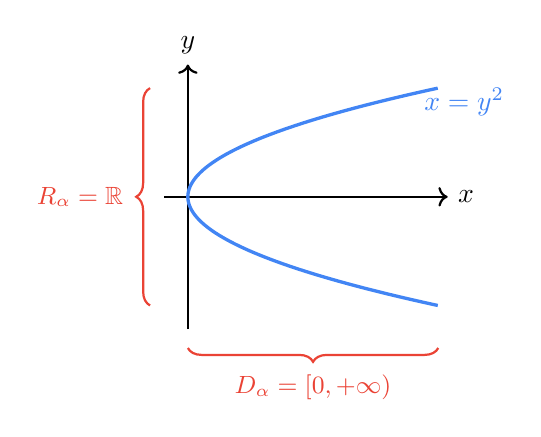
\begin{tikzpicture}[scale=0.6]
  \draw[->, thick] (-0.5,0) -- (5.5,0) node[right] {$x$};
  \draw[->, thick] (0,-2.8) -- (0,2.8) node[above] {$y$};
  \draw[setA, very thick, domain=-2.3:2.3, samples=100] plot ({(\x)^2}, \x);
  \node[setA, right] at (4.8, 2) {$x = y^2$};
  % Braces for D and R
  \draw[thick, setB, decorate, decoration={brace, amplitude=5pt, mirror}]
    (0,-3.2) -- (5.3,-3.2) node[midway, below=6pt, setB] {\small $D_\alpha = [0,+\infty)$};
  \draw[thick, setB, decorate, decoration={brace, amplitude=5pt}]
    (-0.8,-2.3) -- (-0.8,2.3) node[midway, left=6pt, setB] {\small $R_\alpha = \R$};
\end{tikzpicture}
\end{center}

%────────────────────────────────────────
\subsection*{(d)\; $\alpha = \{(x,y) \in \R^2 \mid x^2 + y^2 \le 16\}$}

Սա 4 շառավղով փակ շրջան է՝ կենտրոնացած կոորդինատների սկզբնակետում։
Ցանկացած $x$-ի համար, որտեղ $|x| \le 4$, գոյություն ունի $y$, որը բավարարում է $x^2 + y^2 \le 16$, և հակառակը։

\begin{answerbox}
$D_\alpha = [-4,\, 4], \qquad R_\alpha = [-4,\, 4]։$
\end{answerbox}

\begin{center}
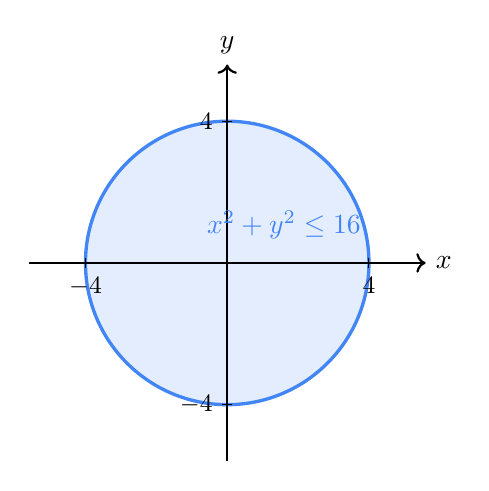
\begin{tikzpicture}[scale=0.6]
  \fill[setA!15] (0,0) circle (3);
  \draw[setA, very thick] (0,0) circle (3);
  \draw[->, thick] (-4.2,0) -- (4.2,0) node[right] {$x$};
  \draw[->, thick] (0,-4.2) -- (0,4.2) node[above] {$y$};
  \foreach \v/\lab in {-3/{-4}, 3/4} {
    \draw (\v, 0.1) -- (\v, -0.1) node[below]{\small $\lab$};
    \draw (0.1, \v) -- (-0.1, \v) node[left]{\small $\lab$};
  }
  \node[setA] at (1.2, 0.8) {$x^2+y^2 \le 16$};
\end{tikzpicture}
\end{center}

%────────────────────────────────────────
\subsection*{(e)\; $\alpha = \{(x,y) \in \N^2 \mid x \le y\}$}

Յուրաքանչյուր $x \in \N$ հարաբերվում է առնվազն $y=x$-ի հետ, ուստի $D_\alpha = \N$։
Յուրաքանչյուր $y \in \N$ հանդես է գալիս որպես երկրորդ կոորդինատ (վերցրեք $x=y$), ուստի $R_\alpha = \N$։

\begin{answerbox}
$D_\alpha = \N, \quad R_\alpha = \N։$
\end{answerbox}

%────────────────────────────────────────
\subsection*{(f)\; $\alpha = \{(x,y) \in \N^2 \mid y \le x\}$}

Նմանապես՝ յուրաքանչյուր $x \in \N$ հարաբերվում է $y=x$-ի հետ, ուստի $D_\alpha = \N$։
Եվ յուրաքանչյուր $y \in \N$-ի համապատասխանում է $x=y$, ուստի $R_\alpha = \N$։

\begin{answerbox}
$D_\alpha = \N, \quad R_\alpha = \N։$
\end{answerbox}

%────────────────────────────────────────
\subsection*{(g)\; $\alpha = \{(x,y) \in \R^2 \mid x + y \ge 0\}$}

Սա $y = -x$ ուղղից վերև և դրա վրա գտնվող կիսահարթությունն է։
Ցանկացած $x \in \R$-ի համար ընտրեք $y = -x + 1$, այդ դեպքում $x + y = 1 \ge 0$։
Ցանկացած $y \in \R$-ի համար ընտրեք $x = -y + 1$։

\begin{answerbox}
$D_\alpha = \R, \quad R_\alpha = \R։$
\end{answerbox}

\begin{center}
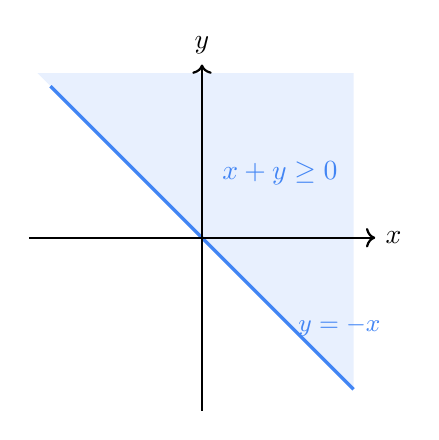
\begin{tikzpicture}[scale=0.55]
  % Shaded half-plane
  \fill[setA!12] (-3.5,3.5) -- (3.5,-3.5) -- (3.5,3.8) -- (-3.8,3.8) -- (-3.5,3.5);
  % Boundary line
  \draw[setA, very thick] (-3.5,3.5) -- (3.5,-3.5);
  % Axes
  \draw[->, thick] (-4,0) -- (4,0) node[right] {$x$};
  \draw[->, thick] (0,-4) -- (0,4) node[above] {$y$};
  \node[setA] at (1.8, 1.5) {$x+y \ge 0$};
  \node[setA, above right] at (2, -2.5) {\small $y=-x$};
\end{tikzpicture}
\end{center}

%────────────────────────────────────────
\subsection*{(h)\; $\alpha = \{(x,y) \in \R^2 \mid 2x \ge 3y\}$}

Համարժեք է $y \le \tfrac{2}{3}\,x$-ին։
Ցանկացած $x$-ի համար ընտրեք $y = 0$ (երբ $x \ge 0$) կամ ցանկացած բավականաչափ փոքր $y$։
Ցանկացած $y$-ի համար ընտրեք $x = \tfrac{3}{2}y$։

\begin{answerbox}
$D_\alpha = \R, \quad R_\alpha = \R։$
\end{answerbox}

% ══════════════════════════════════════════════════════════════════
\newpage
\section{Խնդիր 2.1 — Հարաբերությունների գրաֆ և մատրից}
% ══════════════════════════════════════════════════════════════════

\begin{theorybox}[Հարաբերությունների գրաֆներ և մատրիցներ]
Դիցուք $\alpha$-ն $A = \{a_1,\dots,a_n\}$ վերջավոր բազմության վրա հարաբերություն է։
\begin{itemize}[nosep]
  \item \textbf{Գրաֆ.} $A$-ի յուրաքանչյուր տարր գագաթ է։ Սիմետրիկ հարաբերության համար, եթե $(a_i, a_j) \in \alpha$ և $i \ne j$, տարեք \emph{չուղղորդված} կող $a_i$-ի և $a_j$-ի միջև։
  \item \textbf{Մատրից.} $n \times n$ մատրից $M$, որտեղ $M_{ij} = 1$, եթե $(a_i, a_j) \in \alpha$, և $M_{ij} = 0$ հակառակ դեպքում։ Սիմետրիկ հարաբերության համար $M = M^T$։
\end{itemize}
\end{theorybox}

\begin{problembox}
Կառուցեք գրաֆը և մատրիցը $A = \{a, b, c, d, e\}$ բազմության վրա տրված հետևյալ հարաբերությունների համար։
\end{problembox}

% TikZ style for undirected graph nodes
\tikzset{
  gnode/.style={circle, draw, thick, minimum size=8mm, inner sep=0pt, font=\small},
}

%────────────────────────────────────────
\subsection*{(a)\; $\alpha = \{(a,b),(b,a),(b,c),(c,b),(c,a),(a,c),(d,e),(e,d)\}$}

Քանի որ յուրաքանչյուր զույգ հանդիպում է իր հակառակի հետ, հարաբերությունը սիմետրիկ է։ Չուղղորդված կողեր.
\[
  \boxed{a\text{--}b,\quad b\text{--}c,\quad a\text{--}c,\quad d\text{--}e։}
\]

\begin{center}
\begin{minipage}{0.45\textwidth}\centering
\begin{tikzpicture}
  % Pentagon layout
  \node[gnode] (a) at (90:1.8)  {$a$};
  \node[gnode] (b) at (18:1.8)  {$b$};
  \node[gnode] (c) at (306:1.8) {$c$};
  \node[gnode] (d) at (234:1.8) {$d$};
  \node[gnode] (e) at (162:1.8) {$e$};

  \draw[thick, setA] (a) -- (b);
  \draw[thick, setA] (b) -- (c);
  \draw[thick, setA] (a) -- (c);
  \draw[thick, setA] (d) -- (e);
\end{tikzpicture}
\end{minipage}%
\begin{minipage}{0.5\textwidth}\centering
\textbf{Գունավորված մատրից} (սիմետրիան տեսանելի է)։\\[4pt]
{\small Անկյունագիծ = \colorbox{diagGray}{մոխրագույն},\;
հայելային 1-եր = \colorbox{mirrorBlue}{կապույտ} / \colorbox{mirrorRose}{վարդագույն}։}\\[4pt]
\renewcommand{\arraystretch}{1.15}
$M_\alpha = \left(\;\begin{tabular}{c|ccccc}
  & $a$ & $b$ & $c$ & $d$ & $e$ \\\hline
$a$ & \cellcolor{diagGray}0 & \cellcolor{mirrorBlue}1 & \cellcolor{mirrorRose}1 & 0 & 0 \\
$b$ & \cellcolor{mirrorBlue}1 & \cellcolor{diagGray}0 & \cellcolor{mirrorBlue}1 & 0 & 0 \\
$c$ & \cellcolor{mirrorRose}1 & \cellcolor{mirrorBlue}1 & \cellcolor{diagGray}0 & 0 & 0 \\
$d$ & 0 & 0 & 0 & \cellcolor{diagGray}0 & \cellcolor{mirrorRose}1 \\
$e$ & 0 & 0 & 0 & \cellcolor{mirrorRose}1 & \cellcolor{diagGray}0
\end{tabular}\;\right)$
\end{minipage}
\end{center}

Մատրիցը սիմետրիկ է ($M = M^T$). անկյունագծից վերև գտնվող յուրաքանչյուր ստվերագծված 1-ին համապատասխանում է ներքևում գտնվող ստվերագծված 1։
Երկու կապակցված բաղադրիչներ։ եռանկյունի $\{a,b,c\}$ և կող $\{d,e\}$։

\textbf{Կառուցման կարգ.}\; $A$-ի վրա վերջավոր հարաբերության համար. (1) թվարկեք կարգավորված զույգերը, (2) լրացրեք մատրիցը տող առ տող զույգերից, (3) կարդացեք ուղղորդված գրաֆը մատրիցից։

%────────────────────────────────────────
\subsection*{(b)\; $\alpha = \{(a,b),(b,a),(b,c),(c,b),(c,d),(d,c),(c,a),(a,c)\}$}

Չուղղորդված կողեր.
\[
  \boxed{a\text{--}b,\quad b\text{--}c,\quad c\text{--}d,\quad a\text{--}c։}
\]

\begin{center}
\begin{minipage}{0.45\textwidth}\centering
\begin{tikzpicture}
  \node[gnode] (a) at (90:1.8)  {$a$};
  \node[gnode] (b) at (18:1.8)  {$b$};
  \node[gnode] (c) at (306:1.8) {$c$};
  \node[gnode] (d) at (234:1.8) {$d$};
  \node[gnode] (e) at (162:1.8) {$e$};

  \draw[thick, setA] (a) -- (b);
  \draw[thick, setA] (b) -- (c);
  \draw[thick, setA] (a) -- (c);
  \draw[thick, setA] (c) -- (d);
\end{tikzpicture}
\end{minipage}%
\begin{minipage}{0.5\textwidth}\centering
\renewcommand{\arraystretch}{1.15}
$M_\alpha = \left(\;\begin{tabular}{c|ccccc}
  & $a$ & $b$ & $c$ & $d$ & $e$ \\\hline
$a$ & \cellcolor{diagGray}0 & \cellcolor{mirrorBlue}1 & \cellcolor{mirrorRose}1 & 0 & 0 \\
$b$ & \cellcolor{mirrorBlue}1 & \cellcolor{diagGray}0 & \cellcolor{mirrorBlue}1 & 0 & 0 \\
$c$ & \cellcolor{mirrorRose}1 & \cellcolor{mirrorBlue}1 & \cellcolor{diagGray}0 & \cellcolor{mirrorRose}1 & 0 \\
$d$ & 0 & 0 & \cellcolor{mirrorRose}1 & \cellcolor{diagGray}0 & 0 \\
$e$ & 0 & 0 & 0 & 0 & \cellcolor{diagGray}0
\end{tabular}\;\right)$
\end{minipage}
\end{center}

Եռանկյունի $\{a,b,c\}$, որին կցված է $d$-ն $c$-ի միջոցով; $e$ գագաթը մեկուսացված է։

%────────────────────────────────────────
\subsection*{(c)}

(c) մասը նույնական է (b) մասին սկզբնական խնդրագրքում։ Գրաֆը և մատրիցը նույնն են, ինչ վերևում։

% ══════════════════════════════════════════════════════════════════
\newpage
\section{Խնդիր 2.2 — Հարաբերությունների դիգրաֆ և մատրից}
% ══════════════════════════════════════════════════════════════════

\begin{theorybox}[Ուղղորդված գրաֆներ (Դիգրաֆներ)]
$A$-ի վրա (ոչ անպայման սիմետրիկ) $\alpha$ հարաբերության համար։
\begin{itemize}[nosep]
  \item \textbf{Դիգրաֆ.} Գագաթները $A$-ի տարրերն են։ Յուրաքանչյուր $(a_i,a_j) \in \alpha$-ի համար տարեք սլաք $a_i \to a_j$։ $(a_i,a_i)$ զույգը \emph{օղակ} է։
  \item \textbf{Մատրից.} Նույն կառուցումը; մատրիցը պարտադիր չէ, որ լինի սիմետրիկ։
\end{itemize}
\end{theorybox}

\begin{tcolorbox}[colback=white, colframe=gray!50, arc=2mm, width=0.9\textwidth, halign=center]
  \textbf{Տեսանյութ.} Կառուցել հարաբերության դիգրաֆը և մատրիցը \\
  \href{https://youtu.be/jVi59i_XRBw}{\textbf{[VIDEO]} Դիտել YouTube-ում (ID: jVi59i\_XRBw)}
\end{tcolorbox}

\begin{problembox}
Կառուցեք դիգրաֆը և մատրիցը $A = \{a, b, c, d, e, f\}$ բազմության վրա հետևյալ հարաբերությունների համար։
\end{problembox}

% TikZ style for digraph
\tikzset{
  dnode/.style={circle, draw, thick, minimum size=8mm, inner sep=0pt, font=\small},
  darr/.style={-{Stealth[length=5pt]}, thick, setA},
}

%────────────────────────────────────────
\subsection*{(a)\; $\alpha = \{(a,b),(b,c),(a,c),(b,e),(c,f),(c,d),(d,f),(f,e)\}$}

\begin{center}
\begin{tikzpicture}
  % Layout: top-flow for a→b→c, bottom for e,f,d
  \node[dnode] (a) at (0,2.5)   {$a$};
  \node[dnode] (b) at (2.5,2.5) {$b$};
  \node[dnode] (c) at (5,2.5)   {$c$};
  \node[dnode] (f) at (2.5,0)   {$f$};
  \node[dnode] (e) at (0,0)     {$e$};
  \node[dnode] (d) at (5,0)     {$d$};

  \draw[darr] (a) -- (b);
  \draw[darr] (b) -- (c);
  \draw[darr] (a) edge[bend right=15] (c);
  \draw[darr] (b) edge[bend left=8] (e);
  \draw[darr] (c) -- (f);
  \draw[darr] (c) -- (d);
  \draw[darr] (d) -- (f);
  \draw[darr] (f) -- (e);
\end{tikzpicture}
\end{center}

\[
M_\alpha = \bordermatrix{
  & a & b & c & d & e & f \cr
a & 0 & 1 & 1 & 0 & 0 & 0 \cr
b & 0 & 0 & 1 & 0 & 1 & 0 \cr
c & 0 & 0 & 0 & 1 & 0 & 1 \cr
d & 0 & 0 & 0 & 0 & 0 & 1 \cr
e & 0 & 0 & 0 & 0 & 0 & 0 \cr
f & 0 & 0 & 0 & 0 & 1 & 0 \cr
}
\]

%────────────────────────────────────────
\subsection*{(b)\; $\alpha = \{(a,b),(b,c),(d,c),(d,e),(f,e),(f,a),(b,e)\}$}

\begin{center}
\begin{tikzpicture}
  \node[dnode] (a) at (0,2.5)   {$a$};
  \node[dnode] (b) at (2.5,2.5) {$b$};
  \node[dnode] (c) at (5,2.5)   {$c$};
  \node[dnode] (d) at (5,0)     {$d$};
  \node[dnode] (e) at (2.5,0)   {$e$};
  \node[dnode] (f) at (0,0)     {$f$};

  \draw[darr] (a) -- (b);
  \draw[darr] (b) -- (c);
  \draw[darr] (b) -- (e);
  \draw[darr] (d) -- (c);
  \draw[darr] (d) -- (e);
  \draw[darr] (f) -- (e);
  \draw[darr] (f) -- (a);
\end{tikzpicture}
\end{center}

\[
M_\alpha = \bordermatrix{
  & a & b & c & d & e & f \cr
a & 0 & 1 & 0 & 0 & 0 & 0 \cr
b & 0 & 0 & 1 & 0 & 1 & 0 \cr
c & 0 & 0 & 0 & 0 & 0 & 0 \cr
d & 0 & 0 & 1 & 0 & 1 & 0 \cr
e & 0 & 0 & 0 & 0 & 0 & 0 \cr
f & 1 & 0 & 0 & 0 & 1 & 0 \cr
}
\]

%────────────────────────────────────────
\subsection*{(c)\; $\alpha = \{(a,c),(c,c),(c,d),(c,e),(e,c),(e,e),(e,f),(a,e)\}$}

\begin{center}
\begin{tikzpicture}
  % Reposition: b is isolated, push it aside; cluster active vertices
  \node[dnode] (a) at (0,2)     {$a$};
  \node[dnode] (c) at (3,2)     {$c$};
  \node[dnode] (d) at (5.5,2)   {$d$};
  \node[dnode] (e) at (3,0)     {$e$};
  \node[dnode] (f) at (5.5,0)   {$f$};
  \node[dnode, dashed, gray] (b) at (0,0) {$b$};

  \draw[darr] (a) -- (c);
  \draw[darr] (a) -- (e);
  \draw[darr] (c) edge[loop above, looseness=8, min distance=10mm] (c);
  \draw[darr] (c) -- (d);
  \draw[darr] (c) edge[bend left=12] (e);
  \draw[darr] (e) edge[bend left=12] (c);
  \draw[darr] (e) edge[loop below, looseness=8, min distance=10mm] (e);
  \draw[darr] (e) -- (f);
\end{tikzpicture}
\end{center}

Նշում. $b$ գագաթը (կետագծերով) ամբողջովին մեկուսացված է՝ նրան կողեր չեն դիպչում։

\[
M_\alpha = \bordermatrix{
  & a & b & c & d & e & f \cr
a & 0 & 0 & 1 & 0 & 1 & 0 \cr
b & 0 & 0 & 0 & 0 & 0 & 0 \cr
c & 0 & 0 & 1 & 1 & 1 & 0 \cr
d & 0 & 0 & 0 & 0 & 0 & 0 \cr
e & 0 & 0 & 1 & 0 & 1 & 1 \cr
f & 0 & 0 & 0 & 0 & 0 & 0 \cr
}
\]

$c$-ի և $e$-ի օղակները երևում են որպես 1-եր գլխավոր անկյունագծի վրա։ $b$-ի տողը և $b$-ի սյունակը ամբողջությամբ զրոներ են։

Մատրիցում զրոյական տողը նշանակում է «ելնող կողեր չկան» այդ տարրից։ Զրոյական սյունակը նշանակում է «մտնող կողեր չկան» դեպի այդ տարրը։

%────────────────────────────────────────
\subsection*{Հակադրություն. Սիմետրիկ (2.1) ընդդեմ Ոչ սիմետրիկ (2.2) Մատրիցներ}

Խնդիրներ 2.1-ի և 2.2-ի մատրիցները ցույց են տալիս սիմետրիկ (չուղղորդված) և ընդհանուր (ուղղորդված) հարաբերությունների կառուցվածքային տարբերությունը։ Ստորև մենք տեղադրում ենք 2.1(a)-ի մատրիցը 2.2(a)-ի մատրիցի կողքին։

\begin{center}
\begin{minipage}{0.45\textwidth}\centering
\textbf{Խնդիր 2.1\,(a) — Սիմետրիկ}\\[4pt]
\renewcommand{\arraystretch}{1.15}
$\left(\;\begin{tabular}{ccccc}
0 & 1 & 1 & 0 & 0 \\
1 & 0 & 1 & 0 & 0 \\
1 & 1 & 0 & 0 & 0 \\
0 & 0 & 0 & 0 & 1 \\
0 & 0 & 0 & 1 & 0
\end{tabular}\;\right)$\\[4pt]
{\small $M = M^T$: $(i,j)$ տարրը միշտ հավասար է $(j,i)$ տարրին։\\
Չուղղորդված կողեր; սլաքներ պետք չեն։}
\end{minipage}%
\hfill
\begin{minipage}{0.45\textwidth}\centering
\textbf{Խնդիր 2.2\,(a) — Ոչ սիմետրիկ}\\[4pt]
\renewcommand{\arraystretch}{1.15}
$\left(\;\begin{tabular}{cccccc}
0 & 1 & 1 & 0 & 0 & 0 \\
0 & 0 & 1 & 0 & 1 & 0 \\
0 & 0 & 0 & 1 & 0 & 1 \\
0 & 0 & 0 & 0 & 0 & 1 \\
0 & 0 & 0 & 0 & 0 & 0 \\
0 & 0 & 0 & 0 & 1 & 0
\end{tabular}\;\right)$\\[4pt]
{\small $M \ne M^T$: օր.՝ $M_{12}=1$ բայց $M_{21}=0$.\\
Պահանջվում են ուղղորդված կողեր (սլաքներ)։}
\end{minipage}
\end{center}

%────────────────────────────────────────
\subsection*{Աստիճանի հետևում — Խնդիր 2.2\,(a)}

Ուղղորդված հարաբերության համար յուրաքանչյուր գագաթ ունի \textbf{մուտքային աստիճան} (մտնող կողերի քանակը) և \textbf{ելքային աստիճան} (ելնող կողերի քանակը)։ Դրանք կարդացվում են անմիջապես մատրիցից։ $v$-ի ելքային աստիճանը տողի գումարն է, իսկ մուտքային աստիճանը՝ սյունակի գումարը։

\begin{center}
\renewcommand{\arraystretch}{1.2}
\begin{tabular}{c|c|c}
  \toprule
  \textbf{Գագաթ} & \textbf{Մուտքային աստիճան} & \textbf{Ելքային աստիճան} \\
  \midrule
  $a$ & 0 & 2 \\
  $b$ & 1 & 2 \\
  $c$ & 2 & 2 \\
  $d$ & 1 & 1 \\
  $e$ & 2 & 0 \\
  $f$ & 2 & 1 \\
  \bottomrule
\end{tabular}
\end{center}

Նկատեք, որ $\sum \text{մուտքային աստիճաններ} = \sum \text{ելքային աստիճաններ} = |\alpha| = 8$ (յուրաքանչյուր կող յուրաքանչյուր գումարին ավելացնում է 1)։

$e$ գագաթն ունի 0 ելքային աստիճան, ինչը նրան դարձնում է \emph{կլանիչ} (ելնող սլաքներ չկան)։
$a$ գագաթն ունի 0 մուտքային աստիճան, ինչը նրան դարձնում է \emph{աղբյուր} (մտնող սլաքներ չկան)։

% ══════════════════════════════════════════════════════════════════
\newpage
\section{Խնդիր 3.3 — Հարաբերությունների կոմպոզիցիա}
% ══════════════════════════════════════════════════════════════════

\begin{theorybox}[Հարաբերությունների կոմպոզիցիա]
Դիցուք $\alpha \subseteq A \times B$ և $\beta \subseteq B \times C$։ $\alpha \circ \beta$ \textbf{կոմպոզիցիան} (նաև գրվում է $\alpha \cdot \beta$) հարաբերություն է $A \times C$-ի վրա, որը սահմանվում է։
\[
  (x, z) \in \alpha \circ \beta
  \;\;\Longleftrightarrow\;\;
  \exists\, y \in B:\;
  (x, y) \in \alpha \;\land\; (y, z) \in \beta:
\]
Կարդացեք ձախից աջ։ նախ անցեք $\alpha$-ով ($x$-ից որևէ $y$), այնուհետև $\beta$-ով ($y$-ից $z$)։
\end{theorybox}

\begin{problembox}
Դիցուք $\alpha$ և $\beta$ հարաբերություններ են $\Z$-ի վրա։
\[
  \alpha = \{(x,\, x+2) \mid x \in \Z\}, \qquad
  \beta  = \{(x,\, x-2) \mid x \in \Z\}:
\]
Գտեք $\alpha \circ \beta$ և $\beta \circ \alpha$։
\end{problembox}

\textbf{Պայմանավորվածություն.}\; Հարաբերությունների կոմպոզիցիան այստեղ կարդացվում է \textbf{ձախից աջ}։ $\alpha \circ \beta$-ում նախ կիրառեք $\alpha$-ն, հետո $\beta$-ն։ Սա սխալների ամենատարածված աղբյուրն է։

\medskip

\subsection*{$\alpha \circ \beta$-ի որոշումը}

Նախ կիրառում ենք $\alpha$-ն, ապա՝ $\beta$-ն։
\begin{itemize}[nosep]
  \item $(x, y) \in \alpha \;\Longrightarrow\; y = x + 2$:
  \item $(y, z) \in \beta  \;\Longrightarrow\; z = y - 2 = (x+2)-2 = x$:
\end{itemize}

\begin{answerbox}
$\alpha \circ \beta = \{\,(x,\; x) \mid x \in \Z\,\} = \Delta_{\Z}։$
\end{answerbox}

\subsection*{$\beta \circ \alpha$-ի որոշումը}

Մենք կիրառում ենք $\beta$-ն առաջինը, հետո $\alpha$-ն։
\begin{itemize}[nosep]
  \item $(x, y) \in \beta  \;\Longrightarrow\; y = x - 2$:
  \item $(y, z) \in \alpha \;\Longrightarrow\; z = y + 2 = (x-2)+2 = x$:
\end{itemize}

\begin{answerbox}
$\beta \circ \alpha = \{\,(x,\; x) \mid x \in \Z\,\} = \Delta_{\Z}։$
\end{answerbox}

\subsection*{Ստուգում և համեմատում}

\begin{center}
\renewcommand{\arraystretch}{1.1}
\begin{tabular}{r c c}
  \toprule
  $x$ & $\alpha \circ \beta$ & $\beta \circ \alpha$ \\
  \midrule
  $-2$ & $-2$ & $-2$ \\
  $0$  & $0$  & $0$  \\
  $1$  & $1$  & $1$  \\
  $3$  & $3$  & $3$  \\
  \bottomrule
\end{tabular}
\end{center}

\textbf{Հիմնական դիտարկում.} Այստեղ երկու կոմպոզիցիաներն էլ հավասար են $\Delta_{\Z}$ նույնական հարաբերությանը։ Սա հատուկ դեպք է։ կոմպոզիցիան ընդհանուր դեպքում կոմուտատիվ (տեղափոխական) \emph{չէ}։

\begin{center}
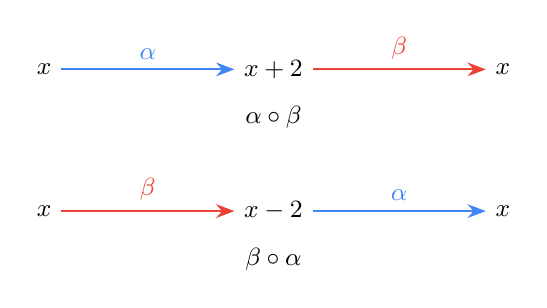
\begin{tikzpicture}[>=Stealth, font=\small, node distance=2.2cm]
  % alpha then beta
  \node (x1) {$x$};
  \node[right=of x1] (y1) {$x+2$};
  \node[right=of y1] (z1) {$x$};
  \draw[->, thick, setA] (x1) -- node[above]{$\alpha$} (y1);
  \draw[->, thick, setB] (y1) -- node[above]{$\beta$} (z1);
  \node[below=3pt of y1] {\small $\alpha \circ \beta$};

  % beta then alpha
  \begin{scope}[yshift=-1.8cm]
  \node (x2) {$x$};
  \node[right=of x2] (y2) {$x-2$};
  \node[right=of y2] (z2) {$x$};
  \draw[->, thick, setB] (x2) -- node[above]{$\beta$} (y2);
  \draw[->, thick, setA] (y2) -- node[above]{$\alpha$} (z2);
  \node[below=3pt of y2] {\small $\beta \circ \alpha$};
  \end{scope}
\end{tikzpicture}
\end{center}

\subsection*{Արտապատկերման դիագրամ վերջավոր օրինակի համար}

Հետագա ինտուիցիայի համար դիտարկենք կոնկրետ վերջավոր օրինակ։
Դիցուք $X = \{1,2,3\}$, $Y = \{a,b\}$, $Z = \{p,q\}$, որտեղ
\[
  R = \{(1,a),\;(2,b),\;(3,a)\} \subseteq X \times Y,
  \qquad
  S = \{(a,p),\;(b,q)\} \subseteq Y \times Z:
\]
Այդ դեպքում $R \circ S$-ը կապում է յուրաքանչյուր $x \in X$-ը յուրաքանչյուր $z \in Z$-ի հետ, որը հասանելի է ինչ-որ միջանկյալ $y$-ի միջոցով։
\[
  \boxed{R \circ S = \{(1,p),\;(2,q),\;(3,p)\}։}
\]

\begin{center}
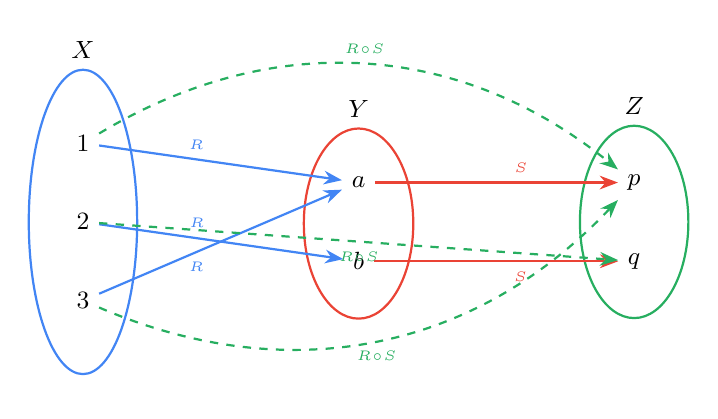
\begin{tikzpicture}[>=Stealth, node distance=0.8cm, font=\small]
  % Set X
  \node (x1) at (0, 2)   {$1$};
  \node (x2) at (0, 1)   {$2$};
  \node (x3) at (0, 0)   {$3$};
  \node[draw=setA, ellipse, thick, fit=(x1)(x2)(x3),
        inner xsep=8pt, inner ysep=4pt, label={above:$X$}] {};

  % Set Y
  \node (ya) at (3.5, 1.5) {$a$};
  \node (yb) at (3.5, 0.5) {$b$};
  \node[draw=setB, ellipse, thick, fit=(ya)(yb),
        inner xsep=8pt, inner ysep=4pt, label={above:$Y$}] {};

  % Set Z
  \node (zp) at (7, 1.5) {$p$};
  \node (zq) at (7, 0.5) {$q$};
  \node[draw=newEdge, ellipse, thick, fit=(zp)(zq),
        inner xsep=8pt, inner ysep=4pt, label={above:$Z$}] {};

  % Relation R (X -> Y)
  \draw[->, thick, setA] (x1) -- node[above, pos=0.4]{\tiny $R$} (ya);
  \draw[->, thick, setA] (x2) -- node[above, pos=0.4]{\tiny $R$} (yb);
  \draw[->, thick, setA] (x3) -- node[below, pos=0.4]{\tiny $R$} (ya);

  % Relation S (Y -> Z)
  \draw[->, thick, setB] (ya) -- node[above, pos=0.6]{\tiny $S$} (zp);
  \draw[->, thick, setB] (yb) -- node[below, pos=0.6]{\tiny $S$} (zq);

  % Composition paths (dashed, green)
  \draw[->, thick, newEdge, dashed, bend left=35]
    (x1) to node[above, pos=0.5]{\tiny $R\!\circ\!S$} (zp);
  \draw[->, thick, newEdge, dashed, bend right=0]
    (x2) to node[below, pos=0.5]{\tiny $R\!\circ\!S$} (zq);
  \draw[->, thick, newEdge, dashed, bend right=35]
    (x3) to node[below, pos=0.5]{\tiny $R\!\circ\!S$} (zp);
\end{tikzpicture}
\end{center}

{\small\textbf{Դիագրամի ընթերցում.} Հոծ կապույտ սլաքները $R$-ն են, հոծ կարմիր սլաքները՝ $S$-ը, իսկ կետագծված կանաչ սլաքները՝ $R \circ S$-ի կոմպոզիցիոն զույգերը։ Յուրաքանչյուր կետագծված սլաք ներկայացնում է կապակցված ճանապարհ $Y$-ի որևէ միջանկյալ գագաթի միջոցով:}

% ══════════════════════════════════════════════════════════════════
\newpage
\section{Խնդիր 4.1 — Հարաբերությունների հատկություններ}
% ══════════════════════════════════════════════════════════════════

\begin{theorybox}[Հարաբերությունների հատկություններ]
$A$ բազմության վրա $\alpha$ հարաբերությունը կարող է բավարարել։
\begin{itemize}[nosep]
  \item \textbf{Ռեֆլեքսիվ.} $\forall x \in A:\; (x,x) \in \alpha$:
  \item \textbf{Սիմետրիկ.} $(x,y) \in \alpha \;\Rightarrow\; (y,x) \in \alpha$:
  \item \textbf{Հակասիմետրիկ.} $(x,y) \in \alpha \;\land\; (y,x) \in \alpha \;\Rightarrow\; x = y$:
  \item \textbf{Տրանզիտիվ.} $(x,y) \in \alpha \;\land\; (y,z) \in \alpha \;\Rightarrow\; (x,z) \in \alpha$:
\end{itemize}
Նշում. սիմետրիկը և հակասիմետրիկը մեկը մյուսի ժխտումը \emph{չեն}։ հարաբերությունը կարող է լինել երկուսն էլ (օր.՝ $\Delta_A$) կամ ոչ մեկը։
\end{theorybox}

\begin{problembox}
Որոշեք, թե որ հատկություններին է բավարարում հետևյալ հարաբերություններից յուրաքանչյուրը։
\end{problembox}

%────────────────────────────────────────
\subsection*{(a)\; $\alpha = \{(x,y) \in \R^2 \mid x^2 + y^2 = 1\}$}

Երկրաչափորեն, $(x,y) \in \alpha$, եթե և միայն եթե $(x,y)$ կետը գտնվում է միավոր շրջանագծի վրա։

\begin{center}
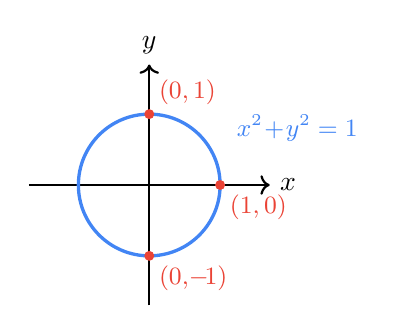
\begin{tikzpicture}[scale=0.9]
  \draw[->, thick] (-1.7,0) -- (1.7,0) node[right] {$x$};
  \draw[->, thick] (0,-1.7) -- (0,1.7) node[above] {$y$};
  \draw[setA, very thick] (0,0) circle (1);
  \fill[setB] (1,0) circle (2pt) node[below right]{\small $(1,0)$};
  \fill[setB] (0,1) circle (2pt) node[above right]{\small $(0,1)$};
  \fill[setB] (0,-1) circle (2pt) node[below right]{\small $(0,\!-\!1)$};
  \node[setA, right] at (1.1, 0.8) {\small $x^2\!+\!y^2=1$};
\end{tikzpicture}
\end{center}

\textbf{Ռեֆլեքսի՞վ։} Ոչ։ Մեզ պետք է $2x^2 = 1$ \emph{բոլոր} $x$-երի համար, ինչը չի բավարարվում $x = 0$-ի դեպքում:

\textbf{Սիմետրի՞կ։} Այո։ $x^2 + y^2 = y^2 + x^2$: \checkmark

\textbf{Հակասիմետրի՞կ։} Ոչ։ $(0, 1) \in \alpha$ և $(1, 0) \in \alpha$, բայց $0 \ne 1$:

\textbf{Տրանզիտի՞վ։} Ոչ։ $(1, 0)$ և $(0, 1) \in \alpha$, բայց $(1, 1) \notin \alpha$, քանի որ $1 + 1 = 2 \ne 1$:

\begin{answerbox}
Միայն սիմետրիկ։
\end{answerbox}

\begin{center}
\renewcommand{\arraystretch}{1.15}
\begin{tabular}{l|c|l}
  \toprule
  \textbf{Հատկություն} & \textbf{Բավարարո՞ւմ է} & \textbf{Հիմնավորում} \\
  \midrule
  Ռեֆլեքսիվ      & Ոչ  & $(0,0)$: $0^2+0^2=0\ne1$ \\
  Սիմետրիկ      & Այո & $x^2+y^2 = y^2+x^2$ \\
  Հակասիմետրիկ  & Ոչ  & $(0,1)$ և $(1,0)$ երկուսն էլ $\in\alpha$, բայց $0\ne1$ \\
  Տրանզիտիվ     & Ոչ  & $(1,0),(0,1)\in\alpha$ բայց $(1,1)\notin\alpha$ \\
  \midrule
  \textbf{Դասակարգում} & \multicolumn{2}{l}{Ոչ համարժեքության հարաբերություն, ոչ մասնակի կարգ} \\
  \bottomrule
\end{tabular}
\end{center}

%────────────────────────────────────────
\subsection*{(b)\; $\alpha = \{(x,y) \in \R^2 \mid x^2 = y^2\}$}

Համարժեքորեն $|x| = |y|$, ուստի $y = \pm x$.

\textbf{Ռեֆլեքսի՞վ։} Այո։ $x^2 = x^2$ միշտ տեղի ունի։ \checkmark

\textbf{Սիմետրի՞կ։} Այո։ $x^2 = y^2 \Rightarrow y^2 = x^2$: \checkmark

\textbf{Հակասիմետրի՞կ։} Ոչ։ $1^2 = (-1)^2$ և $(-1)^2 = 1^2$, բայց $1 \ne -1$:

\textbf{Տրանզիտի՞վ։} Այո։ $x^2 = y^2$ և $y^2 = z^2$ հետևում է $x^2 = z^2$: \checkmark

\begin{answerbox}
Ռեֆլեքսիվ, սիմետրիկ, տրանզիտիվ — սա \textbf{համարժեքության հարաբերություն} է։

Համարժեքության դասեր. $[x] = \{x, -x\}$ յուրաքանչյուր $x \in \R$-ի համար։
\end{answerbox}

\begin{center}
\renewcommand{\arraystretch}{1.15}
\begin{tabular}{l|c|l}
  \toprule
  \textbf{Հատկություն} & \textbf{Բավարարո՞ւմ է} & \textbf{Հիմնավորում} \\
  \midrule
  Ռեֆլեքսիվ      & Այո & $x^2 = x^2$ միշտ \\
  Սիմետրիկ      & Այո & $x^2=y^2 \Rightarrow y^2=x^2$ \\
  Հակասիմետրիկ  & Ոչ  & $1^2=(-1)^2$ և $(-1)^2=1^2$, բայց $1\ne -1$ \\
  Տրանզիտիվ     & Այո & $x^2=y^2, y^2=z^2 \Rightarrow x^2=z^2$ \\
  \midrule
  \textbf{Դասակարգում} & \multicolumn{2}{l}{\textbf{Համարժեքության հարաբերություն}} \\
  \bottomrule
\end{tabular}
\end{center}

\smallskip
\textbf{Մակածված տրոհում.}\; $\R$-ը տրոհվում է $\{x,-x\}$ բլոկների։ $x=0$-ի համար բլոկը $\{0\}$-ն է; $x\ne 0$-ի համար յուրաքանչյուր բլոկ ունի ճիշտ երկու տարր։

%────────────────────────────────────────
\subsection*{(c)\; $\alpha = \{(x,y) \in \Z^2 \mid x \le y\}$}

\textbf{Ռեֆլեքսի՞վ։} Այո։ $x \le x$ բոլոր $x \in \Z$-ի համար։ \checkmark

\textbf{Սիմետրի՞կ։} Ոչ։ $1 \le 2$ բայց $2 \nleq 1$:

\textbf{Հակասիմետրի՞կ։} Այո։ Եթե $x \le y$ և $y \le x$, ապա $x=y$: \checkmark

\textbf{Տրանզիտի՞վ։} Այո։ Եթե $x \le y$ և $y \le z$, ապա $x \le z$: \checkmark

\begin{answerbox}
Ռեֆլեքսիվ, հակասիմետրիկ, տրանզիտիվ — սա \textbf{մասնակի կարգ} է։ Փաստացի, այն \textbf{գծային (լրիվ) կարգ} է $\Z$-ի վրա։
\end{answerbox}

\begin{center}
\renewcommand{\arraystretch}{1.15}
\begin{tabular}{l|c|l}
  \toprule
  \textbf{Հատկություն} & \textbf{Բավարարո՞ւմ է} & \textbf{Հիմնավորում} \\
  \midrule
  Ռեֆլեքսիվ      & Այո & $x \le x$ \\
  Սիմետրիկ      & Ոչ  & $1\le 2$ բայց $2\nleq 1$ \\
  Հակասիմետրիկ  & Այո & $x\le y\land y\le x \Rightarrow x=y$ \\
  Տրանզիտիվ     & Այո & $x\le y\le z \Rightarrow x\le z$ \\
  \midrule
  \textbf{Դասակարգում} & \multicolumn{2}{l}{Գծային (լրիվ) կարգ $\Z$-ի վրա} \\
  \bottomrule
\end{tabular}
\end{center}

%────────────────────────────────────────
\subsection*{(d)\; $\alpha = \{(x,y) \in \N^2 \mid x \le y\}$}

Նույնը (c) մասի հետ, բայց սահմանափակված $\N = \{1, 2, 3, \dots\}$-ով։

\textbf{Ռեֆլեքսի՞վ։} Այո։ $x \le x$: \checkmark

\textbf{Սիմետրի՞կ։} Ոչ։ $1 \le 2$ բայց $2 \nleq 1$:

\textbf{Հակասիմետրի՞կ։} Այո։ Եթե $x \le y$ և $y \le x$, ապա $x=y$: \checkmark

\textbf{Տրանզիտի՞վ։} Այո։ Եթե $x \le y$ և $y \le z$, ապա $x \le z$: \checkmark

\begin{answerbox}
Ռեֆլեքսիվ, հակասիմետրիկ, տրանզիտիվ — սա \textbf{մասնակի կարգ} է։ Փաստացի, այն \textbf{գծային (լրիվ) կարգ} է $\N$-ի վրա։
\end{answerbox}

\begin{center}
\renewcommand{\arraystretch}{1.15}
\begin{tabular}{l|c|l}
  \toprule
  \textbf{Հատկություն} & \textbf{Բավարարո՞ւմ է} & \textbf{Հիմնավորում} \\
  \midrule
  Ռեֆլեքսիվ      & Այո & $x \le x$ \\
  Սիմետրիկ      & Ոչ  & $1\le 2$ բայց $2\nleq 1$ \\
  Հակասիմետրիկ  & Այո & $x\le y\land y\le x \Rightarrow x=y$ \\
  Տրանզիտիվ     & Այո & $x\le y\le z \Rightarrow x\le z$ \\
  \midrule
  \textbf{Դասակարգում} & \multicolumn{2}{l}{Գծային (լրիվ) կարգ $\N$-ի վրա} \\
  \bottomrule
\end{tabular}
\end{center}

%────────────────────────────────────────
\subsection*{(e)\; $\alpha = \{(x,y) \in \N^2 \mid \gcd(x,y) = 1\}$}

$(x,y) \in \alpha$ եթե և միայն եթե $x$-ը և $y$-ը փոխադարձաբար պարզ են։

\textbf{Ռեֆլեքսի՞վ։} Ոչ։ $\gcd(2,2) = 2 \ne 1$:

\textbf{Սիմետրի՞կ։} Այո։ $\gcd(x,y) = \gcd(y,x)$: \checkmark

\textbf{Հակասիմետրի՞կ։} Ոչ։ $\gcd(2,3) = 1$ և $\gcd(3,2) = 1$, բայց $2 \ne 3$:

\textbf{Տրանզիտի՞վ։} Ոչ։ $\gcd(2,3) = 1$ և $\gcd(3,4) = 1$, բայց $\gcd(2,4) = 2 \ne 1$:

\begin{answerbox}
Միայն սիմետրիկ։
\end{answerbox}

\begin{center}
\renewcommand{\arraystretch}{1.15}
\begin{tabular}{l|c|l}
  \toprule
  \textbf{Հատկություն} & \textbf{Բավարարո՞ւմ է} & \textbf{Հիմնավորում} \\
  \midrule
  Ռեֆլեքսիվ      & Ոչ  & $\gcd(2,2)=2\ne 1$ \\
  Սիմետրիկ      & Այո & $\gcd(x,y)=\gcd(y,x)$ \\
  Հակասիմետրիկ  & Ոչ  & $\gcd(2,3)=1$ և $\gcd(3,2)=1$, բայց $2\ne 3$ \\
  Տրանզիտիվ     & Ոչ  & $\gcd(2,3)=1,\;\gcd(3,4)=1$, բայց $\gcd(2,4)=2$ \\
  \midrule
  \textbf{Դասակարգում} & \multicolumn{2}{l}{Ոչ համարժեքության հարաբերություն, ոչ մասնակի կարգ} \\
  \bottomrule
\end{tabular}
\end{center}

%────────────────────────────────────────
\subsection*{(f)\; $\alpha = \{(x,y) \in \Z^2 \mid \gcd(x,y) = 1\}$}

Վերլուծությունը նույնական է (e) մասի հետ, քանի որ $\gcd$-ն կախված է միայն բացարձակ արժեքներից։ Նույն հակաօրինակները կիրառելի են։

\begin{answerbox}
Միայն սիմետրիկ։
\end{answerbox}

\begin{center}
\renewcommand{\arraystretch}{1.15}
\begin{tabular}{l|c|l}
  \toprule
  \textbf{Հատկություն} & \textbf{Բավարարո՞ւմ է} & \textbf{Հիմնավորում} \\
  \midrule
  Ռեֆլեքսիվ      & Ոչ  & $\gcd(2,2)=2\ne 1$ \\
  Սիմետրիկ      & Այո & $\gcd(x,y)=\gcd(y,x)$ \\
  Հակասիմետրիկ  & Ոչ  & $\gcd(2,3)=1$ և $\gcd(3,2)=1$, բայց $2\ne 3$ \\
  Տրանզիտիվ     & Ոչ  & $\gcd(2,3)=1,\;\gcd(3,4)=1$, բայց $\gcd(2,4)=2$ \\
  \midrule
  \textbf{Դասակարգում} & \multicolumn{2}{l}{Ոչ համարժեքության հարաբերություն, ոչ մասնակի կարգ} \\
  \bottomrule
\end{tabular}
\end{center}

%────────────────────────────────────────
\subsection*{Ամփոփիչ աղյուսակ}

\begin{center}
\renewcommand{\arraystretch}{1.3}
\begin{tabular}{l c c c c l}
  \toprule
  \textbf{Հարաբերություն} & \textbf{Ռեֆլ.} & \textbf{Սիմ.} & \textbf{Հակաս.} & \textbf{Տրանզ.} & \textbf{Տիպ} \\
  \midrule
  (a)\; $x^2+y^2=1$ ($\R$)    & —  & \checkmark & —  & — & — \\
  (b)\; $x^2=y^2$ ($\R$)      & \checkmark & \checkmark & — & \checkmark & համարժեքություն \\
  (c)\; $x \le y$ ($\Z$)     & \checkmark & — & \checkmark & \checkmark & գծային կարգ \\
  (d)\; $x \le y$ ($\N$)     & \checkmark & — & \checkmark & \checkmark & գծային կարգ \\
  (e)\; $\gcd=1$ ($\N$)       & —  & \checkmark & — & — & — \\
  (f)\; $\gcd=1$ ($\Z$)       & —  & \checkmark & — & — & — \\
  \bottomrule
\end{tabular}
\end{center}

\textbf{Ինչպես ստուգել (արագ թեստեր).}
\begin{itemize}[nosep]
  \item Ոչ ռեֆլեքսիվ։ գտեք մեկ $x$, որի համար $(x,x) \notin R$։
  \item Ոչ սիմետրիկ։ գտեք $(a,b) \in R$ այնպես, որ $(b,a) \notin R$։
  \item Ոչ հակասիմետրիկ։ գտեք $a \neq b$ այնպես, որ երկուսն էլ՝ $(a,b)$ և $(b,a)$, $R$-ում են։
  \item Ոչ տրանզիտիվ։ գտեք $(a,b), (b,c) \in R$ այնպես, որ $(a,c) \notin R$։
\end{itemize}

% ══════════════════════════════════════════════════════════════════
\newpage
\section{Խնդիր 7.2 — Հարաբերության փակումներ}
% ══════════════════════════════════════════════════════════════════

\begin{theorybox}[Հարաբերության փակումներ]
Դիցուք $\alpha$-ն $A$ վերջավոր բազմության վրա հարաբերություն է։
\begin{itemize}[nosep]
  \item \textbf{Ռեֆլեքսիվ փակում} $r(\alpha) = \alpha \cup \Delta_A$, որտեղ $\Delta_A = \{(x,x) \mid x \in A\}$։
  \item \textbf{Սիմետրիկ փակում} $s(\alpha) = \alpha \cup \alpha^{-1}$, որտեղ $\alpha^{-1} = \{(y,x) \mid (x,y) \in \alpha\}$։
  \item \textbf{Տրանզիտիվ փակում} $t(\alpha) = \alpha \cup \alpha^2 \cup \alpha^3 \cup \cdots$\; (բոլոր աստիճանների միավորումը մինչև նոր զույգեր չհայտնվեն)։
\end{itemize}
Փակումն ավելացնում է այն \emph{նվազագույն} զույգերը, որոնք անհրաժեշտ են տվյալ հատկությունը ձեռք բերելու համար։
\end{theorybox}

\begin{problembox}
Դիցուք $A = \{1, 2, 3, 4\}$ և $\alpha = \{(1,2),\,(3,1),\,(3,2),\,(2,4)\}$։

Գտեք $r(\alpha)$, $s(\alpha)$ և $t(\alpha)$։
\end{problembox}

\subsection*{Սկզբնական հարաբերությունը}

\begin{center}
\begin{minipage}{0.45\textwidth}\centering
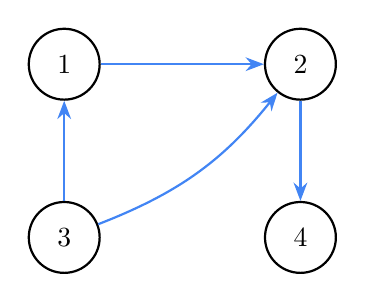
\begin{tikzpicture}[
  every node/.style={circle, draw, thick, minimum size=9mm, inner sep=0pt},
  >=Stealth
]
  \node (1) at (0,2.2)   {$1$};
  \node (2) at (3,2.2)   {$2$};
  \node (3) at (0,0)     {$3$};
  \node (4) at (3,0)     {$4$};

  \draw[->, thick, setA] (1) -- (2);
  \draw[->, thick, setA] (3) -- (1);
  \draw[->, thick, setA] (3) edge[bend right=15] (2);
  \draw[->, thick, setA] (2) -- (4);
\end{tikzpicture}
\end{minipage}%
\begin{minipage}{0.45\textwidth}\centering
$M_\alpha = \begin{pmatrix}
  0 & 1 & 0 & 0 \\
  0 & 0 & 0 & 1 \\
  1 & 1 & 0 & 0 \\
  0 & 0 & 0 & 0
\end{pmatrix}$

{\small Տողեր/սյունակներ՝ $1,2,3,4$:}
\end{minipage}
\end{center}

%────────────────────────────────────────
\subsection*{Ռեֆլեքսիվ փակում $r(\alpha)$}

Ավելացրեք բոլոր անկյունագծային զույգերը $(x,x)$՝ $x \in A$-ի համար։
\begin{align*}
  r(\alpha) &= \alpha \cup \{(1,1),\,(2,2),\,(3,3),\,(4,4)\} \\
            &= \boxed{\{(1,1),\,(1,2),\,(2,2),\,(2,4),\,(3,1),\,(3,2),\,(3,3),\,(4,4)\}։}
\end{align*}

\begin{center}
\begin{minipage}{0.45\textwidth}\centering
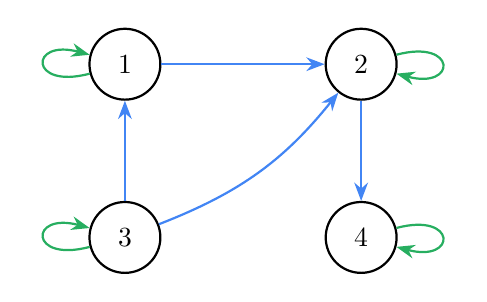
\begin{tikzpicture}[
  every node/.style={circle, draw, thick, minimum size=9mm, inner sep=0pt},
  >=Stealth
]
  \node (1) at (0,2.2)   {$1$};
  \node (2) at (3,2.2)   {$2$};
  \node (3) at (0,0)     {$3$};
  \node (4) at (3,0)     {$4$};

  % Original edges (blue)
  \draw[->, thick, setA] (1) -- (2);
  \draw[->, thick, setA] (3) -- (1);
  \draw[->, thick, setA] (3) edge[bend right=15] (2);
  \draw[->, thick, setA] (2) -- (4);
  % Added loops (green)
  \draw[->, thick, newEdge] (1) edge[loop left, looseness=8, min distance=8mm] (1);
  \draw[->, thick, newEdge] (2) edge[loop right, looseness=8, min distance=8mm] (2);
  \draw[->, thick, newEdge] (3) edge[loop left, looseness=8, min distance=8mm] (3);
  \draw[->, thick, newEdge] (4) edge[loop right, looseness=8, min distance=8mm] (4);
\end{tikzpicture}
\end{minipage}%
\begin{minipage}{0.45\textwidth}\centering
$M_{r(\alpha)} = \begin{pmatrix}
  \mathbf{1} & 1 & 0 & 0 \\
  0 & \mathbf{1} & 0 & 1 \\
  1 & 1 & \mathbf{1} & 0 \\
  0 & 0 & 0 & \mathbf{1}
\end{pmatrix}$

{\small\color{newEdge} Թավ = անկյունագծի վրա ավելացված 1-եր։}
\end{minipage}
\end{center}

%────────────────────────────────────────
\subsection*{Սիմետրիկ փակում $s(\alpha)$}

Ավելացրեք յուրաքանչյուր զույգի հակառակը։
\[
  \alpha^{-1} = \{(2,1),\,(1,3),\,(2,3),\,(4,2)\}:
\]
\[
  \boxed{s(\alpha) = \alpha \cup \alpha^{-1}
  = \{(1,2),\,(1,3),\,(2,1),\,(2,3),\,(2,4),\,(3,1),\,(3,2),\,(4,2)\}։}
\]

\begin{center}
\begin{minipage}{0.45\textwidth}\centering
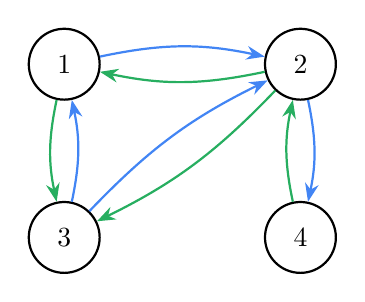
\begin{tikzpicture}[
  every node/.style={circle, draw, thick, minimum size=9mm, inner sep=0pt},
  >=Stealth
]
  \node (1) at (0,2.2)   {$1$};
  \node (2) at (3,2.2)   {$2$};
  \node (3) at (0,0)     {$3$};
  \node (4) at (3,0)     {$4$};

  % Original edges (blue) -- bend to make room for reverse
  \draw[->, thick, setA] (1) edge[bend left=12] (2);
  \draw[->, thick, setA] (3) edge[bend right=12] (1);
  \draw[->, thick, setA] (3) edge[bend left=10] (2);
  \draw[->, thick, setA] (2) edge[bend left=12] (4);
  % Added reverse edges (green)
  \draw[->, thick, newEdge] (2) edge[bend left=12] (1);
  \draw[->, thick, newEdge] (1) edge[bend right=12] (3);
  \draw[->, thick, newEdge] (2) edge[bend left=10] (3);
  \draw[->, thick, newEdge] (4) edge[bend left=12] (2);
\end{tikzpicture}
\end{minipage}%
\begin{minipage}{0.45\textwidth}\centering
$M_{s(\alpha)} = \begin{pmatrix}
  0 & 1 & \mathbf{1} & 0 \\
  \mathbf{1} & 0 & \mathbf{1} & 1 \\
  1 & 1 & 0 & 0 \\
  0 & \mathbf{1} & 0 & 0
\end{pmatrix}$

{\small\color{newEdge} Թավ = ավելացված 1-եր ($M$-ը այժմ սիմետրիկ է)։}
\end{minipage}
\end{center}

%────────────────────────────────────────
\subsection*{Տրանզիտիվ փակում $t(\alpha)$}

\textbf{Մեկնաբանություն.}\; $t(\alpha)$ տրանզիտիվ փակումը ավելացնում է բոլոր $(a,c)$ զույգերը, որոնց համար հարաբերության գրաֆում կա ուղղորդված ճանապարհ $a$-ից դեպի $c$։ Համարժեքորեն, $(a,c) \in t(\alpha)$ եթե և միայն եթե $a$-ն կարող է հասնել $c$-ին մեկ կամ ավելի քայլերով։

\medskip

\begin{tcolorbox}[colback=yellow!5, colframe=stmtFrame!80, arc=2mm,
  fonttitle=\bfseries, title={\small Տեսողական կառուցում. «Կարճ ճանապարհ» կողերի ավելացում},
  breakable, left=5pt, right=5pt, top=4pt, bottom=4pt]
Տրանզիտիվ փակումը կառուցվում է շերտ առ շերտ։ Յուրաքանչյուր քայլում մենք փնտրում ենք աճող երկարությամբ ճանապարհներ և ավելացնում ենք ուղիղ «կարճ ճանապարհ» կող յուրաքանչյուրի համար։

\begin{center}
\begin{tikzpicture}[
  every node/.style={circle, draw, thick, minimum size=9mm, inner sep=0pt},
  >=Stealth
]
  % --- Layer 0: Original relation ---
  \begin{scope}[local bounding box=L0]
    \node (a1) at (0,2.2)   {$1$};
    \node (a2) at (2.5,2.2) {$2$};
    \node (a3) at (0,0)     {$3$};
    \node (a4) at (2.5,0)   {$4$};
    \draw[->, thick, setA] (a1) -- (a2);
    \draw[->, thick, setA] (a3) -- (a1);
    \draw[->, thick, setA] (a3) edge[bend right=12] (a2);
    \draw[->, thick, setA] (a2) -- (a4);
  \end{scope}
  \node[draw=none, below=2pt of L0, font=\small\bfseries] {Քայլ 0: $\alpha$ (սկզբնական)};

  % --- Layer 1: Add length-2 shortcuts ---
  \begin{scope}[xshift=5.5cm, local bounding box=L1]
    \node (b1) at (0,2.2)   {$1$};
    \node (b2) at (2.5,2.2) {$2$};
    \node (b3) at (0,0)     {$3$};
    \node (b4) at (2.5,0)   {$4$};
    % Original edges
    \draw[->, thick, setA] (b1) -- (b2);
    \draw[->, thick, setA] (b3) -- (b1);
    \draw[->, thick, setA] (b3) edge[bend right=12] (b2);
    \draw[->, thick, setA] (b2) -- (b4);
    % New shortcut edges (length-2 paths) -- dashed red
    \draw[->, thick, setB, dashed] (b1) edge[bend left=30] (b4);
    \draw[->, thick, setB, dashed] (b3) -- (b4);
  \end{scope}
  \node[draw=none, below=2pt of L1, font=\small\bfseries] {Քայլ 1: ավելացնել $\alpha^2$ կարճ ճանապարհներ};

  % Legend
  \node[draw=none, font=\small, text width=4cm, align=left]
    at (8.8, 2.8) {%
      \textcolor{setA}{\rule{10pt}{2pt}} սկզբնական ($\alpha$)\\
      \textcolor{setB}{- - -} երկարություն-2 կարճ ճանապարհներ ($\alpha^2$)};
\end{tikzpicture}
\end{center}

\smallskip
Այս օրինակում $4$ գագաթը կլանիչ է (ելնող կողեր չկան), ուստի չկան 3 երկարությամբ ճանապարհներ, որոնք նոր զույգեր կառաջացնեն։ Գործընթացն ավարտվում է։ $t(\alpha) = \alpha \cup \alpha^2$։

Ընդհանուր դեպքում, $|A|=n$-ի համար գործընթացը միշտ ավարտվում է առավելագույնը $n-1$ քայլից հետո, քանի որ $n$-գագաթանի գրաֆում ցանկացած ճանապարհ, որը չի կրկնում գագաթները, ունի $\le n-1$ երկարություն։
\end{tcolorbox}

\medskip

Մենք հաշվարկում ենք $\alpha$-ի հաջորդական աստիճանները։

\textbf{Քայլ 1. $\alpha^2 = \alpha \circ \alpha$։}\; Յուրաքանչյուր $x \xrightarrow{\alpha} y \xrightarrow{\alpha} z$ շղթայի համար։
\begin{itemize}[nosep]
  \item $(1,2)$ և $(2,4)$։ տալիս է $\boldsymbol{(1,4)}$։  \textbf{Նոր է!}
  \item $(3,1)$ և $(1,2)$։ տալիս է $(3,2)$։  Արդեն կա $\alpha$-ում։
  \item $(3,2)$ և $(2,4)$։ տալիս է $\boldsymbol{(3,4)}$։  \textbf{Նոր է!}
\end{itemize}
Նոր զույգեր։ $\boxed{(1,4) \text{ և } (3,4)}$։

\textbf{Քայլ 2. $\alpha^3 = \alpha^2 \circ \alpha$։}\; Նոր երկրորդ կոորդինատները բոլորը $4$ են, բայց $4$-ը $\alpha$-ում չունի ելնող կողեր, ուստի այլևս նոր զույգեր չեն առաջանում։

\begin{answerbox}
$t(\alpha) = \alpha \cup \alpha^2 = \{(1,2),\;(1,4),\;(2,4),\;(3,1),\;(3,2),\;(3,4)\}։$
\end{answerbox}

\textbf{Մեկնաբանություն.} $(x, z) \in t(\alpha)$ եթե և միայն եթե սկզբնական դիգրաֆում կա ուղղորդված ճանապարհ $x$-ից դեպի $z$։

\begin{center}
\begin{minipage}{0.45\textwidth}\centering
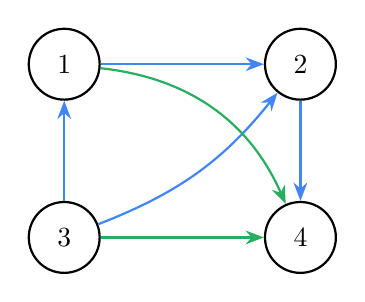
\begin{tikzpicture}[
  every node/.style={circle, draw, thick, minimum size=9mm, inner sep=0pt},
  >=Stealth
]
  \node (1) at (0,2.2)   {$1$};
  \node (2) at (3,2.2)   {$2$};
  \node (3) at (0,0)     {$3$};
  \node (4) at (3,0)     {$4$};

  % Original edges (blue)
  \draw[->, thick, setA] (1) -- (2);
  \draw[->, thick, setA] (3) -- (1);
  \draw[->, thick, setA] (3) edge[bend right=15] (2);
  \draw[->, thick, setA] (2) -- (4);
  % Added transitive edges (green)
  \draw[->, thick, newEdge] (1) edge[bend left=30] (4);
  \draw[->, thick, newEdge] (3) -- (4);
\end{tikzpicture}
\end{minipage}%
\begin{minipage}{0.45\textwidth}\centering
$M_{t(\alpha)} = \begin{pmatrix}
  0 & 1 & 0 & \mathbf{1} \\
  0 & 0 & 0 & 1 \\
  1 & 1 & 0 & \mathbf{1} \\
  0 & 0 & 0 & 0
\end{pmatrix}$

{\small\color{newEdge} Թավ = ավելացված 1-եր։}
\end{minipage}
\end{center}

\medskip

\textbf{Հասանելիության ամփոփում.}
\begin{itemize}[nosep]
  \item $1$-ից կարելի է հասնել $2$ և $4$ \;(ճանապարհ՝ $1 \to 2 \to 4$)։
  \item $2$-ից կարելի է հասնել $4$։
  \item $3$-ից կարելի է հասնել $1$, $2$, և $4$ \;(ճանապարհ՝ $3 \to 1 \to 2 \to 4$)։
  \item $4$-ից ելնող կողեր չկան — $4$-ը \emph{կլանիչ} է։
\end{itemize}

\end{document}